\documentclass[a4paper,11pt]{article}
\usepackage[utf8]{inputenc}
\usepackage{geometry}
\usepackage{xcolor}
\usepackage{hyperref}
\usepackage{amsmath}
\usepackage{amssymb}
\usepackage{tcolorbox}
\usepackage{booktabs}
\usepackage{array}
\usepackage{tikz}

% Page geometry (tighter than the online guides: bench budget of 3 + 2 pages)
\geometry{top=1.8cm, bottom=1.8cm, left=2cm, right=2cm}
\hypersetup{pdftitle={Lab 10: Quantum Optics on the Bench}, colorlinks=true, linkcolor=ibmblue, urlcolor=ibmblue}
\pagestyle{plain}
\setlength{\parindent}{0pt}
\setlength{\parskip}{3pt}

% Custom colours
\definecolor{ibmblue}{RGB}{0, 45, 156}
\definecolor{ibmred}{RGB}{250, 75, 76}
\definecolor{purpleaccent}{RGB}{109, 40, 217}
\definecolor{amberaccent}{RGB}{245, 158, 11}
\definecolor{tealaccent}{RGB}{13, 148, 136}
\definecolor{shockorange}{RGB}{234, 88, 12}

% Custom boxes (titles always in braced form)
\newtcolorbox{studentbox}{colback=blue!5!white,colframe=blue!75!black,title={Student Activity}}
\newtcolorbox{theorybox}{colback=gray!5!white,colframe=gray!50!black,title={Theory Recap}}
\newtcolorbox{warningbox}{colback=yellow!10!white,colframe=orange!80!black,title={Important}}
\newtcolorbox{simulatorbox}{colback=purple!5!white,colframe=purple!75!black,title={Simulator}}
\newtcolorbox{reflectionbox}{colback=teal!5!white,colframe=teal!75!black,title={Quick Check}}
\newtcolorbox{connectionbox}{colback=green!5!white,colframe=green!60!black,title={Connections to Previous Labs}}
\newtcolorbox{procedurebox}{colback=red!4!white,colframe=red!70!black,title={Procedure 1 vs Procedure 2}}
\newtcolorbox{questionbox}{colback=violet!4!white,colframe=violet!70!black,title={The Question}}
\newtcolorbox{shockbox}{colback=shockorange!8!white,colframe=shockorange,title={Counterintuitive --- and Real}}
\newtcolorbox{benchbox}{colback=teal!6!white,colframe=tealaccent,title={Open the Simulator First}}
\newtcolorbox{numberbox}{colback=green!4!white,colframe=green!50!black,title={Formula $\rightarrow$ Number $\rightarrow$ Bench}}
\newtcolorbox{industrybox}{colback=amberaccent!10!white,colframe=amberaccent!90!black,title={Real-World Anchors}}
\newtcolorbox{deepdivebox}{colback=cyan!4!white,colframe=cyan!60!black,title={Deep Dive}}

% Titled variants for this guide (same colour schemes as above)
\newtcolorbox{devbox}[1]{colback=yellow!10!white,colframe=orange!80!black,title={#1}}
\newtcolorbox{labelbox}[1]{colback=gray!5!white,colframe=gray!50!black,title={#1}}
\newtcolorbox{demobox}[1]{colback=cyan!4!white,colframe=cyan!60!black,title={#1}}
\newtcolorbox{pmcbox}[1]{colback=blue!5!white,colframe=blue!75!black,title={#1}}

% Compact spacing for every box (look unchanged)
\tcbset{left=4pt, right=4pt, top=2pt, bottom=2pt, boxsep=2pt,
        before skip=5pt, after skip=5pt, fonttitle=\bfseries\small}

% Bra-ket shorthands (guarded: never clash with package-provided macros)
\providecommand{\ket}[1]{|#1\rangle}
\providecommand{\bra}[1]{\langle#1|}
\providecommand{\braket}[2]{\langle#1|#2\rangle}

% Correlation numbers: \gtwo{HBT} = g^(2)_HBT
\newcommand{\gtwo}[1]{g^{(2)}_{\mathrm{#1}}}

% Section headings: each Part heading is its question
\makeatletter
\renewcommand\section{\@startsection{section}{1}{\z@}{-1.6ex \@plus -.5ex}{0.6ex}{\normalfont\large\bfseries\color{ibmblue}}}
\makeatother

% Compact lists (no enumitem)
\newenvironment{steps}{\begin{enumerate}\setlength{\itemsep}{1pt}\setlength{\parsep}{0pt}\setlength{\topsep}{2pt}}{\end{enumerate}}

% Worksheet cells
\newcolumntype{Y}[1]{>{\rule[-1.9mm]{0pt}{6mm}\centering\arraybackslash\footnotesize}p{#1}}
\newcommand{\blank}[1]{\rule{#1}{0.4pt}}

\begin{document}

% =====================================================================
% === Header ===
% =====================================================================
{\LARGE\bfseries\color{ibmblue} Lab 10: Quantum Optics on the Bench}\par
\vspace{2pt}
{\large Single photons on a tabletop kit}\hfill
\textbf{1 ECTS}\,$\cdot$\,in person at i-LAMP\par
\vspace{4pt}
\textbf{Prerequisites:} \textit{Fundamental Concepts of Quantum Technologies} (lecture
series) --- nothing else.\\
\textbf{What you need:} the Thorlabs EDU-QOP1 Quantum Optics Kit with its time tagger and
software (set up by the staff); the worksheet (pages 4--5); a pen and a calculator.\\
\textbf{Time:} about 10\,h, indicative: Part A 2\,h, B 1.5\,h, C 2\,h, D 2.5\,h, optional
parts 2\,h.\\
{\footnotesize\textbf{Source:} Thorlabs, \textit{EDU-QOP1(/M) Quantum Optics Kit User Guide},
Rev.~D (2025-10-25), ``manual \S x''; follow its sections, this guide does not repeat them.}\\
\textbf{Goal:} decide, from detector clicks alone, whether the light on the bench comes as
single photons, and whether one photon can interfere with itself.

\begin{center}
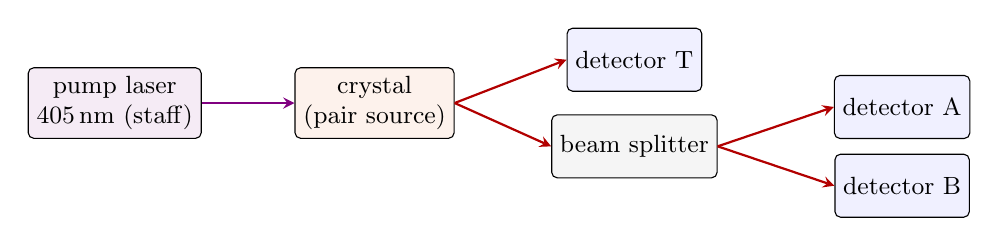
\begin{tikzpicture}[font=\small, >=stealth,
  mod/.style={draw, rounded corners=2pt, align=center, minimum height=8mm, inner sep=3pt}]
  \node[mod, fill=violet!8] (P) at (0,0) {pump laser\\ 405\,nm (staff)};
  \node[mod, fill=shockorange!8] (C) at (3.3,0) {crystal\\ (pair source)};
  \node[mod, fill=blue!6] (T) at (6.6,0.55) {detector T};
  \node[mod, fill=gray!8] (S) at (6.6,-0.55) {beam splitter};
  \node[mod, fill=blue!6] (A) at (10,-0.05) {detector A};
  \node[mod, fill=blue!6] (B) at (10,-1.05) {detector B};
  \draw[->, thick, violet] (P) -- (C);
  \draw[->, thick, red!70!black] (C.east) -- (T.west);
  \draw[->, thick, red!70!black] (C.east) -- (S.west);
  \draw[->, thick, red!70!black] (S.east) -- (A.west);
  \draw[->, thick, red!70!black] (S.east) -- (B.west);
\end{tikzpicture}\\[-1pt]
{\footnotesize Parts B--D. A: dimmed 635\,nm alignment laser into the beam splitter, no T. D: Michelson before B.}
\end{center}

\begin{devbox}{Safety first}
The room is dark during measurements. The 405\,nm pump laser is class 3B: \textbf{only the
staff switch it on} (key, interlock; manual Ch.~1, Ch.~14). While it is on (Parts B--D) you follow the i-LAMP
eyewear and conduct rules of the laser safety officer; the manual is explicit: ``Always wear
laser safety glasses when working with the pump laser!'' (manual \S7.6.4). You use the
635\,nm alignment laser and the software.
\end{devbox}

\begin{labelbox}{Words you need}
\small
\textbf{Beam splitter:} a half-transparent mirror with two outputs (course document QC10,
\textit{Light}).
\textbf{Click:} one pulse of a single-photon detector. \textbf{Coincidence:} two (or three)
detectors click in the same \textbf{window} $\Delta t$ (5\,ns here, set in the software).
$\boldsymbol{g^{(2)}}$\textbf{:} with $P(X)$ the probability that detector $X$ clicks in
one window, $P(X) = R_X\,\Delta t$ for a click rate $R_X$ (clicks per second),
\[ g^{(2)} = \frac{P(A \text{ and } B)}{P(A)\,P(B)}: \quad
   1 = \text{no correlation},\quad {<}\,1 = \text{fewer coincidences than chance},\quad
   {>}\,1 = \text{more}. \]
\textbf{Accidentals:} the coincidences expected by pure chance if A and B click
independently, rate $R_A R_B\,\Delta t$; so $g^{(2)}$ = coincidences / accidentals.
\textbf{Poisson light:} photons arriving independently at random times, like raindrops; a
laser, however dim, is Poisson light. \textbf{Pair source:} a crystal that, pumped at
405\,nm, emits two photons (about 810\,nm) at once. \textbf{Heralding:} a click at T
announces that its partner photon is on the way to the beam splitter; A and B are counted
only together with T. \textbf{Interference:} a wave split in two and recombined adds up or
cancels, depending on the path difference; \textbf{visibility}
$\mathcal{V} = (R_{\max} - R_{\min})/(R_{\max} + R_{\min})$, 1 for perfect fringes.
\textbf{Standard deviation} $\sigma$: the typical scatter of repeated results; a count of
$N$ clicks scatters by about $\sqrt{N}$.
\end{labelbox}

% =====================================================================
% === Part A ===
% =====================================================================
\section*{Part A --- Is a very dim laser a single-photon source?}

A single photon cannot split: at the beam splitter it reaches A \emph{or} B, never both, so
a true single-photon source gives $g^{(2)} = 0$. Poisson light is different: each photon
picks its exit on its own, so A and B click independently and $g^{(2)} = 1$ exactly, at
\emph{every} brightness. The alignment laser is dimmed by the kit's filter; you look at A
and B (Hanbury Brown--Twiss, HBT).

\begin{numberbox}
$\gtwo{HBT} = \dfrac{R_{AB}}{R_A R_B\,\Delta t}$. Manual \S9.1, Table~1 ($\Delta t = 5$\,ns):
accidentals $R_A R_B\,\Delta t = 617.9$\,Hz, measured $R_{AB} = 619.1$\,Hz, so
$\gtwo{HBT} = 1.0020$ (the manual prints 1.00201).
\end{numberbox}

\begin{pmcbox}{Predict $\rightarrow$ measure $\rightarrow$ compare (worksheet W1)}
\textbf{Predict} $g^{(2)}$. \textbf{Measure} following manual \S9.1 (HBT tab, \S11.7):
its 20\,s measurement, three times at the kit's setting. \textbf{Compare} with 1, with
Table~1 (1.0020), and run to run. Dimmer light only enlarges the error bar (manual fn.~84):
try it in the pre-lab playbox.
\end{pmcbox}

\begin{shockbox}
Manual \S9.1 estimates how many photons are inside the 1\,m setup at any moment:
$n = l f / c = 1\,\text{m} \times 1.2\cdot10^{6}\,\text{s}^{-1} / 3\cdot10^{8}\,\text{m\,s}^{-1}
= \mathbf{0.004}$ photons. Far below one --- surely single photons? Yet
$g^{(2)} \approx 1$ (Table~1: 1.0020), not 0. Rare photons are not single photons: a dim
laser stays Poisson.
\end{shockbox}

% =====================================================================
% === Part B ===
% =====================================================================
\section*{Part B --- Does the crystal really make pairs?}

The staff switch on the pump. If the crystal makes pairs, T and A click together far more
often than by chance.

\begin{numberbox}
$\gtwo{PS} = \dfrac{R_{TA}}{R_T R_A\,\Delta t}$ = coincidences / accidentals. Manual
\S9.4, Table~2 (rates = counts / 20\,s): $R_T = 231900$\,Hz, $R_A = 145250$\,Hz,
$R_{TA} = 19293.25$\,Hz, so $\gtwo{PS} \approx 115$: coincidences are
$\approx 115\times$ the accidentals. Table~2 prints no $\Delta t$; we assume the standard
$\Delta t = 5$\,ns (manual \S7.4.5).
\end{numberbox}

\begin{pmcbox}{Predict $\rightarrow$ measure $\rightarrow$ compare (worksheet W2)}
\textbf{Predict:} the manual expects $\gtwo{PS} \ge 30$ (\S9.2). \textbf{Measure} following
manual \S9.2: Alignment tab (manual \S9.2 calls it Adjustment; \S11.5) or GRA tab
(\S11.7), detectors T and A. \textbf{Compare} with 30 and with Table~2.
\end{pmcbox}

% =====================================================================
% === Part C ===
% =====================================================================
\section*{Part C --- Can one photon take both exits?}

Now the partner photon, heralded by T, meets the beam splitter (Grangier--Roger--Aspect,
GRA). Any classical light obeys $g^{(2)} \ge 1$ (manual eq.~75); one photon gives 0. The
software counts a triple as a \emph{coincidence of coincidences}: T\&A and T\&B both
coincident (manual \S4.2.2, \S12.2.1).

\begin{numberbox}
$\gtwo{GRA} = \dfrac{N_{TAB}\,N_T}{N_{TA}\,N_{TB}}$ (counts: the measurement time cancels).
Manual \S9.4, Table~2 (20\,s): $N_T = 4.638$\,M, $N_{TA} = 385865$, $N_{TB} = 324688$,
$N_{TAB} = 513$, so $\gtwo{GRA} = 0.0190$. With
$\sigma \approx \gtwo{GRA}/\sqrt{N_{TAB}} = 0.00084$, it lies
$(1 - \gtwo{GRA})/\sigma \approx 1170$ standard deviations below the classical bound.
\end{numberbox}

\begin{pmcbox}{Predict $\rightarrow$ measure $\rightarrow$ compare (worksheet W3)}
\textbf{Predict:} $\gtwo{GRA} < 1$. \textbf{Measure} following manual \S9.4 (GRA tab,
\S11.7): four counts and the time. \textbf{Compare:} how many $\sigma$ below 1? Is the
residual chance (next box)?
\end{pmcbox}

% DEV-10.2: finite window, accidentals, Poisson pair counts per window
\begin{devbox}{The bench is not the model: the window $\Delta t$}
Detectors and time tagger resolve time only to about a nanosecond, so coincidences are
counted in a window, and unrelated clicks in the same window count too. Two chance types
fake triples (manual eqs.~105--106): $R^{(3)} = R_T R_A R_B\,\Delta t^2$ and
$R^{(2+1)} = (R_{TA} R_B + R_{TB} R_A)\,\Delta t$, giving
$g^{(2)}_{\mathrm{acc}} = (R^{(3)} + R^{(2+1)})\,R_T/(R_{TA} R_{TB})$. Table~2:
$g^{(2)}_{\mathrm{acc}} = 0.0193$, that is $\approx 520$ chance triples in 20\,s against
513 measured, a difference of 0.33\,$\sigma$. \textbf{The residual $\gtwo{GRA}$ is
consistent with chance coincidences alone: no sign of the photon splitting.} A shorter window or weaker pump lowers it (eq.~110).
\end{devbox}

% DEV-10.3: idealized model; efficiency cancels except the herald's in g2_GRA; dark counts and stray light = accidentals
\begin{devbox}{The bench is not the model: real detectors}
Our model is idealized. Detector efficiency cancels in every $g^{(2)}$, except that of the
herald T in $\gtwo{GRA}$: a T that misses photons raises its small two-pair term by up to a
factor 2 (it stays far below 1). Dark counts and stray light enter only as accidentals.
\end{devbox}

% =====================================================================
% === Part D ===
% =====================================================================
\section*{Part D --- Does a single photon interfere with itself?}

The staff place a Michelson interferometer in one beam-splitter output, with B behind it: a
second beam splitter sends the photon into two arms, mirrors send it back, and the arms
recombine. The stage moves one mirror by $x$; the light goes out and back, so the path
difference is $2x$. The detector-side probability is
$P_d(x) = \bigl(1 - \cos(4\pi x/\lambda)\bigr)/2$, so $R_{TB}$ rises and falls with period
$\lambda/2$ in mirror position, while $\gtwo{GRA} < 1$ along the scan.

\begin{numberbox}
With $\lambda \approx 810$\,nm the fringe period is $\approx 405$\,nm in mirror position
(manual \S11.9: ``about 400\,nm''). Backwards, one maximum per fringe:
$\lambda = 2\times$(mean spacing of maxima) $= 2(x_{\mathrm{last}} - x_{\mathrm{first}})/(N_{\max} - 1)
\approx 810$\,nm, with a stage error of up to 3\,\% (manual \S9.7).
\end{numberbox}

\begin{pmcbox}{Predict $\rightarrow$ measure $\rightarrow$ compare (worksheet W4)}
\textbf{Predict} the period and $\lambda$. \textbf{Measure} following manual \S9.7
(Michelson tab, \S11.9); read $\gtwo{GRA}$ during the scan. \textbf{Compare} $\lambda$ with
810\,nm $\pm$ 3\,\%, and $\mathcal{V}$ with 1. Is $\gtwo{GRA} < 1$ at every position? Then
the fringes are built photon by photon.
\end{pmcbox}

% =====================================================================
% === Optional ===
% =====================================================================
\begin{demobox}{Optional (not needed for the core): Parts E, F and two controls}
\footnotesize
\textbf{Polarization} is the direction in which the light's field oscillates; a
\textbf{polarizer} passes one direction; a \textbf{half-wave plate} mirrors the direction
about its axis. The pair photons are vertically polarized.
\textbf{E, quantum eraser} (manual \S7.7, \S9.8): a half-wave plate at $22.5^\circ$ between the
two beam splitters makes the polarization diagonal. Arm polarizers crossed at $0^\circ$ and
$90^\circ$ mark the path: no fringes, $P_d = \tfrac14$ flat. A polarizer at $\pm45^\circ$
before the detector erases the mark and the fringes return,
$P_d = (1 \pm \cos\varphi)/8$ with $\varphi = 4\pi x/\lambda$; with both arm polarizers at $0^\circ$ the maximum is twice
the flat level. \textbf{F, Malus's law for single photons} (manual \S9.6): a polarizer at
$\theta$ from the horizontal passes a heralded photon with probability $\sin^2\theta$.
\textbf{Controls.} Manual \S9.3, one arm alone (T blocked): \emph{thermal light} (many
independent emitters, whose photons bunch) would give 2, but its coherence time
($\approx 0.2$\,ps) is far below $\Delta t$, so expect $\approx 1$, not 2. Manual \S9.5,
GRA with classical light: expect $\approx 1$; three detectors alone do not make
$g^{(2)} < 1$.
\end{demobox}

% DEV-10.1: the plan promises entangled states; the base kit makes |VV> pairs
\begin{devbox}{What this kit cannot show: entanglement}
The course plan promises entangled photons. This kit's single crystal makes pairs with both
photons vertically polarized, $\ket{VV} = \ket{V}\otimes\ket{V}$: ``correlated in time and
energy (though not polarization-entangled)'' (manual Ch.~2). \emph{Entangled} means a
two-photon state that cannot be written as $\ket{\alpha}\otimes\ket{\beta}$, such as
$\ket{\Phi^+} = (\ket{HH} + \ket{VV})/\sqrt{2}$ ($H$: horizontal). The optional notebook
section compares the two with a polarizer on each photon: at the standard angles the CHSH sum $S$ (a combination of four polarizer correlations,
defined in the optional notebook section) is
$S = \sqrt{2} \approx 1.41$ for $\ket{VV}$ against $2\sqrt{2} \approx 2.83$ for
$\ket{\Phi^+}$, while every \emph{local hidden variable model} (each photon leaves the
source with ready-made answers for every polarizer angle) obeys $|S| \le 2$. The Thorlabs
\textit{EDU-QOPA1(/M) Polarization-Entanglement Extension Kit} adds a crossed type-I BBO
pair plus compensation crystals; it is not used here. \emph{Anchor:} the Micius satellite
sent entangled pairs to two ground stations (2017).
\end{devbox}

\begin{industrybox}
\textbf{A:} Hanbury Brown and Twiss (1956) correlated two detectors' signals, the method
behind $\gtwo{HBT}$; it measured the sizes of stars. \textbf{C:} Grangier, Roger and Aspect
(1986) ran Part C with heralded photons from atoms and found 0.18; today Quandela builds
quantum-dot single-photon sources for photonic quantum computers. \textbf{D:} LIGO's
kilometre-long Michelson interferometers reported gravitational waves (2016).
\textbf{Optional:} Nobel Prize in Physics 2022 (Aspect, Clauser, Zeilinger), entangled
photons.
\end{industrybox}

{\footnotesize\textbf{References.} Thorlabs, \textit{EDU-QOP1(/M) Quantum Optics Kit User
Guide}, Rev.~D (2025-10-25): Ch.~1, 2, 14; \S4.2.2, \S7.6.4, \S7.7, \S9.1--9.8, \S11.7, \S11.9,
\S12.2.1. Course document QC10, \textit{Light}. R.~Hanbury Brown, R.~Q.~Twiss,
\textit{Nature} \textbf{177}, 27 (1956). P.~Grangier, G.~Roger, A.~Aspect,
\textit{Europhys.\ Lett.} \textbf{1}, 173 (1986). J.~F.~Clauser, M.~A.~Horne, A.~Shimony,
R.~A.~Holt, \textit{Phys.\ Rev.\ Lett.} \textbf{23}, 880 (1969). Nobel Prize in Physics 2022
(Aspect, Clauser, Zeilinger). J.~Yin et al., \textit{Science} \textbf{356}, 1140 (2017).
B.~P.~Abbott et al., \textit{Phys.\ Rev.\ Lett.} \textbf{116}, 061102 (2016). N.~Somaschi et
al., \textit{Nat.\ Photon.} \textbf{10}, 340 (2016).\par}

% =====================================================================
% === Worksheet ===
% =====================================================================
\newpage
\setlength{\tabcolsep}{3pt}
{\large\bfseries\color{ibmblue} Worksheet --- Lab 10: Quantum Optics on the Bench}\par
{\small Group \blank{1.5cm}\quad Names \blank{8.5cm}\quad Date \blank{2.5cm}}

\vspace{4pt}
\textbf{W1 \,$\cdot$\, Part A: attenuated laser (HBT), kit setting, 20\,s per run.}
{\small $\Delta t$ = \blank{1.2cm} ns. Rates in Hz; accidentals $= R_A R_B\,\Delta t$;
$\gtwo{HBT} = R_{AB}$ / accidentals.}\\[2pt]
\begin{tabular}{|Y{2.4cm}|Y{2cm}|Y{2cm}|Y{1.7cm}|Y{2.2cm}|Y{1.9cm}|Y{2cm}|}\hline
run & $R_A$ & $R_B$ & $R_{AB}$ & accidentals & $\gtwo{HBT}$ & predicted \\ \hline
run 1 & & & & & & 1 \\ \hline
run 2 & & & & & & 1 \\ \hline
run 3 & & & & & & 1 \\ \hline
\multicolumn{7}{|l|}{\footnotesize\emph{Optional:} extra ND filter (only if i-LAMP has one; tens of minutes per run)} \\ \hline
extra ND filter & & & & & & 1 \\ \hline
\end{tabular}\\[3pt]
{\small\textbf{Compare:} Table~1 gives 1.0020. Your runs: consistent with 1 and with each
other? \blank{4cm}}

\vspace{6pt}
\textbf{W2 \,$\cdot$\, Part B: pair source.}
{\small $\gtwo{PS} = R_{TA}/(R_T R_A\,\Delta t)$.}\\[2pt]
\begin{tabular}{|Y{2.4cm}|Y{2cm}|Y{2cm}|Y{1.7cm}|Y{2.2cm}|Y{1.9cm}|Y{2cm}|}\hline
 & $R_T$ & $R_A$ & $R_{TA}$ & $R_T R_A\,\Delta t$ & $\gtwo{PS}$ & predicted \\ \hline
your run & & & & & & $\ge 30$ \\ \hline
\end{tabular}\\[3pt]
{\small\textbf{Compare:} at least 30? Table~2 gives $\approx 115$. \blank{9cm}}

\vspace{6pt}
\textbf{W3 \,$\cdot$\, Part C: heralded photons (GRA).}
{\small $\gtwo{GRA} = N_{TAB} N_T/(N_{TA} N_{TB})$;\quad $\sigma \approx \gtwo{GRA}/\sqrt{N_{TAB}}$.
The Table~2 row is the manual's example.}\\[2pt]
\begin{tabular}{|Y{2.4cm}|Y{1.2cm}|Y{1.5cm}|Y{1.5cm}|Y{1.5cm}|Y{1.2cm}|Y{1.4cm}|Y{1.5cm}|Y{1.6cm}|}\hline
 & time (s) & $N_T$ & $N_{TA}$ & $N_{TB}$ & $N_{TAB}$ & $\gtwo{GRA}$ & $\sigma$ & $(1-g^{(2)})/\sigma$ \\ \hline
Table 2 & 20 & 4.638\,M & 385865 & 324688 & 513 & 0.0190 & 0.00084 & 1170 \\ \hline
your run & & & & & & & & \\ \hline
predicted & \multicolumn{5}{c|}{\footnotesize one photon cannot take both exits} & ${<}\,1$ & & \\ \hline
\end{tabular}\\[4pt]
{\small\textbf{Accidentals (the window box).} Rates $R_X = N_X/\text{time}$ in Hz;\quad
$R^{(3)} = R_T R_A R_B\,\Delta t^2$;\quad $R^{(2+1)} = (R_{TA} R_B + R_{TB} R_A)\,\Delta t$;\quad
$g^{(2)}_{\mathrm{acc}} = (R^{(3)} + R^{(2+1)})\,R_T/(R_{TA} R_{TB})$;\quad
chance triples $= (R^{(3)} + R^{(2+1)})\times$time.}\\[2pt]
\begin{tabular}{|Y{2.4cm}|Y{2.4cm}|Y{2.4cm}|Y{2.4cm}|Y{2.4cm}|Y{2.4cm}|}\hline
 & $R_T$ & $R_A$ & $R_B$ & $R_{TA}$ & $R_{TB}$ \\ \hline
Table 2 & 231900 & 145250 & 146250 & 19293.25 & 16234.4 \\ \hline
your run & & & & & \\ \hline
\end{tabular}\\[2pt]
\begin{tabular}{|Y{2.4cm}|Y{2.4cm}|Y{2.4cm}|Y{2.4cm}|Y{2.4cm}|Y{2.4cm}|}\hline
 & $R^{(3)}$ (Hz) & $R^{(2+1)}$ (Hz) & $g^{(2)}_{\mathrm{acc}}$ & chance triples & $\dfrac{\text{chance} - N_{TAB}}{\sqrt{N_{TAB}}}$ \\ \hline
Table 2 & 0.1232 & 25.898 & 0.0193 & 520 & 0.33 \\ \hline
your run & & & & & \\ \hline
\end{tabular}\\[3pt]
{\small\textbf{Compare:} is $\gtwo{GRA}$ below 1 by many $\sigma$? Do chance triples explain
your $N_{TAB}$? \blank{4.6cm}}

% --- worksheet page 2 ---
\newpage
\textbf{W4 \,$\cdot$\, Part D: heralded Michelson.}
{\small Positions $x$ of the fringe maxima of $R_{TB}$ (in $\mu$m), in order; one maximum per fringe.
Record at least the first and the last, and count them all for $N_{\max}$.}\\[2pt]
\begin{tabular}{|Y{1.55cm}|*{10}{Y{1.25cm}|}}\hline
maximum & 1 & 2 & 3 & 4 & 5 & 6 & 7 & 8 & 9 & 10 \\ \hline
$x$ ($\mu$m) & & & & & & & & & & \\ \hline
maximum & 11 & 12 & 13 & 14 & 15 & 16 & 17 & 18 & 19 & 20 \\ \hline
$x$ ($\mu$m) & & & & & & & & & & \\ \hline
\end{tabular}\\[3pt]
\begin{tabular}{|Y{2.4cm}|Y{1.3cm}|Y{1.6cm}|Y{1.6cm}|Y{2.2cm}|Y{1.5cm}|Y{1.4cm}|Y{1.4cm}|Y{1.2cm}|}\hline
 & $N_{\max}$ & $x_{\mathrm{first}}$ & $x_{\mathrm{last}}$ & spacing (nm) & $\lambda$ (nm) & $R_{\max}$ & $R_{\min}$ & $\mathcal{V}$ \\ \hline
your scan & & & & & & & & \\ \hline
predicted & & & & $\approx 405$ & $\approx 810$ & & & 1 (ideal) \\ \hline
\end{tabular}\\[3pt]
{\small $\lambda = 2(x_{\mathrm{last}} - x_{\mathrm{first}})/(N_{\max} - 1)$.\quad
$\gtwo{GRA}$ at a maximum \blank{1.3cm}, a minimum \blank{1.3cm}, in between \blank{1.3cm}
(predicted: all ${<}\,1$).\\
\textbf{Compare:} is $\lambda$ within 3\,\% of 810\,nm? \blank{8.5cm}}

\vspace{6pt}
\textbf{W5 \,$\cdot$\, Optional parts.}\\[2pt]
\begin{tabular}{|Y{3.4cm}|Y{1.3cm}|Y{1.3cm}|Y{1.3cm}|Y{1.3cm}|Y{1.3cm}|Y{5.2cm}|}\hline
F: polarizer $\theta$ & $0^\circ$ & $30^\circ$ & $45^\circ$ & $60^\circ$ & $90^\circ$ & \\ \hline
predicted $\sin^2\theta$ & 0 & $\tfrac14$ & $\tfrac12$ & $\tfrac34$ & 1 & \\ \hline
measured (relative) & & & & & & \\ \hline
\end{tabular}\\[3pt]
\begin{tabular}{|Y{3.4cm}|Y{3.2cm}|Y{3.4cm}|Y{3.2cm}|}\hline
E: eraser & arms crossed & crossed $+$ $\pm45^\circ$ & both arms $0^\circ$ \\ \hline
predicted & no fringes & fringes & fringes \\ \hline
observed & & & \\ \hline
\end{tabular}\\[3pt]
\begin{tabular}{|Y{3.4cm}|Y{4.2cm}|Y{4.2cm}|}\hline
controls & one arm alone (\S9.3) & classical GRA (\S9.5) \\ \hline
predicted $g^{(2)}$ & $\approx 1$ & $\approx 1$ \\ \hline
measured $g^{(2)}$ & & \\ \hline
\end{tabular}

\end{document}
